%auto-ignore
%
\providecommand{\MainFolder}{..}
\documentclass[\MainFolder/Text.tex]{subfiles}
\begin{document}

\section{String topology and Chen's iterated integrals}

String topology of a manifold~$M$ is the study of the \emph{free loop space} 
\[ \Loop M = \{\gamma: \Sph{1}\rightarrow M\text{ continuous}\} \]
with the compact-open topology and natural structures on it. Each loop~$\gamma$ is parametrized, with base-point~$1$, and there is a natural $\Sph{1}$-action changing the base-point. Therefore, we distinguish two homology theories:
\begin{center}
\begin{tabular}{rl}
 $\H(\Loop M)\quad\dotsc$& the \emph{singular homology} and \\[1ex]
 $\H^{\Sph{1}}\!(\Loop M)\quad\dotsc$ & \parbox[t]{10cm}{the \emph{equivariant homology} --- ``the singular homology of the space of parametrized loops with the base-point forgotten.''}
\end{tabular}
\end{center}
In this thesis, we consider $\H^{\Sph{1}}\!(\Loop M)$ with coefficients in $\R$ only.

If $M=\Sigma$ is an oriented surface, we consider immersed loops with transverse double points and define a bracket and cobracket by Figure~\ref{Fig:ConstrLoop}.
%\footnote{If one wishes, and is allowed to, one can cut holes inside of the loops and make some non-contractible.}
\begin{figure}[t]
\begin{equation*}
\begin{aligned}
\StringOp_2\left(
\parbox[c]{2.85cm}{
\begin{tikzpicture}
	\def\rad{.8cm}
	\draw[green,dashed,thick,decoration={markings, mark=at position 0.25 with {\arrow{>}}},postaction={decorate}] ([shift=(0:\rad)]0,0) arc (0:360:\rad);  
	%\draw[green,thick,dotted] ([shift=(280:\rad)]0,0) arc (280:360:\rad);
	\draw[red,thick,decoration={markings, mark=at position 0.25 with {\arrow{>}}},postaction={decorate}] (1.5*\rad,0) circle (\rad);
	\end{tikzpicture}}
\right)
&=\parbox[c]{2.85cm}{
\begin{tikzpicture}
	\def\rad{.8cm}
	\draw[blue,thick] ([shift=(90:\rad)]0,0) arc (90:360:\rad); %Big loop on the lft
    \draw[blue,thick] ([shift=(0:\rad)]0,0) arc (0:180:.25*\rad); %Small connecting loop
	\draw[blue,thick] ([shift=(180:\rad)]1.5*\rad,0) arc (180:450:\rad); %Big loop on the right
	\draw[blue,thick,decoration={markings, mark=at position 0.5 with {\arrow{<}}},
        postaction={decorate}] ([shift=(90:\rad)]0,0) to ([shift=(90:\rad)]1.5*\rad,0); %The oriented connecting line
\end{tikzpicture}}
\ -\ 
\parbox[c]{2.85cm}{
\begin{tikzpicture}
	\def\rad{.8cm}
	\draw[blue,thick] ([shift=(0:\rad)]0,0) arc (0:270:\rad); %Big loop on the left
	\draw[blue,thick] ([shift=(180:\rad)]1.5*\rad,0) arc (180:360:.25*\rad); %Small connecting loop
	\draw[blue,thick] ([shift=(270:\rad)]1.5*\rad,0) arc (270:540:\rad); %Big loop on the right
	\draw[blue,thick,decoration={markings, mark=at position 0.5 with {\arrow{>}}},
        postaction={decorate}] ([shift=(270:\rad)]0,0) to ([shift=(270:\rad)]1.5*\rad,0);
\end{tikzpicture}}\\
\StringCoOp_2\left(\hspace{-.4em}
\parbox[c]{3.3cm}{
\begin{tikzpicture}
	\def\rad{.8cm}
	\draw[blue,thick,decoration={markings, mark=at position 0.25 with {\arrow{>}}},
        postaction={decorate}] ([shift=(45:\rad)]0,0) arc (45:315:\rad);
	\draw[blue,thick,decoration={markings, mark=at position 0.25 with {\arrow{<}}},
        postaction={decorate}] ([shift=(-135:\rad)]2*\rad,0) arc (-135:135:\rad);
	\draw[blue,thick] (45:\rad) to[out=-45,in=135] ($(-135:\rad)+(2*\rad,0)$);
	\draw[blue,thick] (-45:\rad) to[out=45,in=225] ($(135:\rad)+(2*\rad,0)$);
\end{tikzpicture}}\right)
&=\parbox[c]{1.64cm}{
\begin{tikzpicture}
\def\rad{.8cm}
\draw[green,thick,dashed,decoration={markings, mark=at position 0.25 with {\arrow{>}}},
        postaction={decorate}] (0,0) circle (\rad);
\end{tikzpicture}}\otimes
\parbox[c]{1.64cm}{
\begin{tikzpicture}
\def\rad{.8cm}
\draw[red,thick,decoration={markings, mark=at position 0.25 with {\arrow{<}}},
        postaction={decorate}] (0,0) circle (\rad);
\end{tikzpicture}}\ -\ 
\parbox[c]{1.64cm}{
\begin{tikzpicture}
\def\rad{.8cm}
\draw[red,thick,decoration={markings, mark=at position 0.25 with {\arrow{<}}},
        postaction={decorate}] (0,0) circle (\rad);
\end{tikzpicture}} \otimes
\parbox[c]{1.64cm}{
\begin{tikzpicture}
\def\rad{.8cm}
\draw[green,dashed,thick,decoration={markings, mark=at position 0.25 with {\arrow{>}}},
        postaction={decorate}] (0,0) circle (\rad);
\end{tikzpicture}}
\end{aligned}
\end{equation*}
\caption[Bracket and cobracket in equivariant string topology.]{Bracket and cobracket in equivariant string topology. Imagine some genus so that the operations are homotopically non-trivial.}
\label{Fig:ConstrLoop}
\end{figure}
In words:\ToDo[noline,caption={How is it with loop parametrization}]{How is it precisely with the speeds?}
\begin{description}[leftmargin=*]
 \item[$\StringOp_2$:] Imagine putting one base-point $b_1$ on the first loop $\gamma_1$ and another base-point $b_2$ on the second loop $\gamma_2$ in all possible positions. Whenever $\gamma_1(b_1) = \gamma_2(b_2) = p$, construct a new loop~$\gamma = \gamma_1 \Star_p \gamma_2$ by running first along $\gamma_1$ with double speed starting and ending at~$b_1$ and continuing along $\gamma_2$ starting and ending at $b_2$. Forget the base-points and multiply $\gamma$ with the sign of the intersection $\varepsilon(p;\gamma_1, \gamma_2)$. Should more intersections occur, take the sum.
 \item[$\StringCoOp_2$:] Imagine putting the basepoints $b_1$ and $b_2$ on $\gamma$ in all possible positions such that $b_1 \neq b_2$. Whenever $\gamma(b_1) = \gamma(b_2)=p$, split $\gamma$ into~$\gamma_1$ and $\gamma_2$ as follows. The first loop~$\gamma_1$ is the portion of~$\gamma$ from $b_1$ to $b_2$ and the second loop $\gamma_2$ is the portion from $b_2$ to $b_1$ ran along with the correspondingly scaled speed. Forget the base-points, form the tensor product $\gamma_1 \otimes \gamma_2$ and multiply it with $\varepsilon(p; \gamma)$. Should more self-intersections occur, take the sum of the tensors.
\end{description}
The operations $\StringOp_2$ and $\StringCoOp_2$ are known as the \emph{Goldman bracket} and the \emph{Turaev cobracket} and were defined and studied in \cite{Goldman1986} and \cite{Turaev1991}, respectively.

In \cite{Sullivan1999}, it was demonstrated that the construction of~$\StringOp_2$ extends to families of loops and to an arbitrary dimension~$n$ of an oriented manifold~$M$; it produces a Lie bracket on the equivariant homology. The construction of $\StringCoOp_2$ generalizes too, which is explained for instance in \cite{Cieliebak2007}, and gives a Lie cobracket. The picture is always~\ref{Fig:ConstrLoop}, just the intersection points come from transverse intersections of smooth parameter spaces of points on loops in $M$; thus, both $\StringOp_2$ and $\StringCoOp_2$ have degrees $2-n$. Another definition of the coproduct is in \cite{Basu2011}, where loops in $M$ are viewed as open strings in $M\times M$ with endpoints at the diagonal. In order to make these geometric constructions rigorous, the most straightforward way is to use a \emph{geometric homology theory} of $M$ based on smooth chains, so that the transverse intersection of two smooth chains is again a smooth chain. Such theory for smooth manifolds was constructed in \cite{Lipyanskiy2014}. A~version for general topological spaces is proposed in \cite{Cieliebak2013}, and some details regarding triangulations are addressed in~\cite{Hajek2014} (see also the discussion at \cite{MO157762}). Note that $\StringOp_2$ and $\StringCoOp_2$ are only ``transversally defined'' on the chain level and for the definition on homology it is important that we can homotop to a generic situation within the homology class.

The main theorem of \cite{Sullivan2002} asserts that $\StringOp_2$ and $\StringCoOp_2$ induce the structure of an \emph{involutive bi-Lie algebra} (abbreviated $\IBL$) of degree $2-n$ on the equivariant homology $H^{\Sph{1}}\!(\Loop M,M)$ relative to constant loops $M\xhookrightarrow{}\Loop M$. Modding out constant loops is necessary for $\StringCoOp_2$ to be well defined because of the phenomenon of \emph{``vanishing of small loops''} illustrated in~\cite{Cieliebak2007}:  Let $\sigma\in C_1(\Loop M)$ be a $1$-chain supported at $[0,1]$ which for $t=0$ agrees with the loop in the argument of $\StringCoOp_2$ in \ref{Fig:ConstrLoop}, for $t\in (0,1)$ the left knot $L$ contracts to the mid-point $p$ (thus the name) and for $t=1$ only the right knot $R$ remains. It is then easy to see that 
\[ 0 \neq \Bdd \StringCoOp_2(\sigma) - \StringCoOp_2(\Bdd \sigma) = p\otimes R - L \otimes p \in C(M)\otimes C(\Loop M) + C(\Loop M)\otimes C(M). \]
%In fact, there might be another problem with the restriction of $\StringOp_2$ to $H^{\Sph{1}}\!(\Loop M,M)$ as constant loops might not form an ideal (this is easy to see for $M=\T^2$).
The string bracket $\StringOp_2$ restricts to a Lie bracket on the relative homology because applied to a chain of constant loops it gives a degenerate chain.\footnote{This is in contrast to the situation on the non-equivariant homology $\H(\Loop M)$, where constant loops do not always form an ideal for the associative loop product; this is easy to see in the case of the torus $\T^2$. They do, however, provided that the Euler characteristics $\chi(M)$ is non-zero (see \cite{Tamanoi2010}). On the other hand, if $\chi(M)=0$, then the loop coproduct admits an extension to $\H(\Loop M)$, which is possibly dependent on the choice of a non-vanishing vector field (see \cite{Basu2011}).}
%Our current understanding of this issue is that there should be an $\IBL$-structure either on $\H^{\Sph{1}}\!(\Loop M)$, if the Euler characteristics $\chi(M)$ vanishes, or on the homology $\H^{\Sph{1}}\!(\Loop M,\mathrm{pt})$ relative to one point, if $\chi(M) \neq 0$. However, the extension of $\StringCoOp_2$ requires choices (of a nowhere vanishing vector field, see \cite{Basu2011}), and it is not clear to which extent the $\IBL$-structure depends on it.
In the work in progress~\cite{CieliebakHingston2018}, Poincar\'e duality on the Rabinowitz-Floer homology of the unit cotangent bundle of $M$ is introduced and related to the (non-equivariant) string topology via a long exact sequence. This shall give a canonical extension of $\StringCoOp_2$ to $\H^{\Sph{1}}\!(\Loop M,\mathrm{pt})$, the relative homology modulo one point, which together with $\StringOp_2$ makes $\H^{\Sph{1}}\!(\Loop M,\mathrm{pt})$ into a bi-Lie algebra (in fact, this is what our chain model computes). We will use $\RedEquivHom(\Loop M)$ as an avatar for either $\H^{\Sph{1}}\!(\Loop M,M)$ or $\H^{\Sph{1}}\!(\Loop M,\mathrm{pt})$.

It is expected that the $\IBL$-structure on $\RedEquivHom(\Loop M)$ is induced from a much richer (and in some context natural) algebraic structure on the chain level whose homotopy type is an invariant of $M$. In fact, there is the notion of a \emph{strong homotopy involutive bi-Lie algebra} (abbreviated $\IBLInfty$) which was developed in~\cite{Cieliebak2015}. It consists of operations $(\OPQ_{klg})$ for $k$, $l \ge 1$ and $g\ge 0$, where $\OPQ_{110}$ is a boundary operator, $\OPQ_{210}$ a bracket and $\OPQ_{120}$ a cobracket, which satisfy the $\IBL$-relations up to a coherent system of higher homotopies~$(\OPQ_{klg})$. Consider the string space 
\[ \StringSpace M \coloneqq (\EG\Sph{1}\times \Loop M)/\Sph{1} \]
(the homotopically correct version of the quotient $\Loop M/\Sph{1}$), and let $(C(\StringSpace M),\Bdd)$ be the singular chain complex of $\StringSpace M$ where~$\StringOp_2$ and $\StringCoOp_2$ are partially defined on transverse smooth chains. An \emph{$\IBLInfty$-chain model for equivariant string topology} is an $\IBLInfty$-algebra $(\Model(\StringSpace M),(\OPQ_{klg}))$ ($\Model$ stands for ``model'') together with a weak homotopy equivalence  ($\coloneqq$~zig-zag of quasi-isomorphisms) of $(C(\StringSpace M),\Bdd)$ and $(\Model(\StringSpace M),\OPQ_{110})$ which induces an isomorphism of $\IBL$-algebras
\[ (\RedEquivHom(\Loop M),\StringOp_2,\StringCoOp_2) \simeq (\H(\Model(\StringSpace M),\OPQ_{110}), \OPQ_{210}, \OPQ_{120}). \]
Note that there can be various non-homotopically equivalent $\IBLInfty$-chain models. On the other hand, the properad $\IBLInfty$ is a quasi-free resolution of the properad $\IBL$ and as such has convenient homotopy theoretical properties, e.g., homotopy inverses of quasi-isomorphisms exist. These properties imply that any two weakly homotopy equivalent $\IBLInfty$-algebras are (strongly) homotopy equivalent.


In this thesis, we use a version of \emph{perturbative Chern-Simons theory} to construct an $\IBLInfty$-chain model for the equivariant string topology starting with an oriented compact Riemannian manifold~$M$. Chains are cyclic Hochschild cochains of the de Rham cohomology $\HDR$ of $M$, and the homotopy type of the model is supposed to be an invariant of~$M$ (perhaps topological). As the construction involves a version of Feynman integrals, the proof of well-definedness relies on Stokes' theorem on compactifications of configuration spaces, which is currently being developped in \cite{Cieliebak2018} and~\cite{Cieliebak2018b}. The concrete form of this chain model was sketched in \cite{Cieliebak2015}. It is expected that the evaluation at boundaries of pseudo-holomorphic curves in the compactification induces an $\IBLInfty$-quasi-isomorphism of the SFT of the unit cotangent bundle of $M$ and the $\IBLInfty$-chain model of string topology, see~\cite{Cieliebak2007}.

We now describe the underlying chain complex and the quasi-isomorphism to string topology in more details. Let $\BCyc \DR$, where $\DR$ is the space of de Rham forms on $M$, be the graded vector space generated by cyclic words 
\[ \omega_1\dotsb\omega_k = (-1)^{\Abs{\omega_k}(\Abs{\omega_1}+\dotsb+\Abs{\omega_k})} \omega_k\omega_1 \dotsb \omega_{k-1} \]
with homogenous $\omega_1$, $\dotsc$, $\omega_k \in \DR$ for $k\ge 1$. The grading satisfies $\Abs{\omega_i} = \Deg(\omega_i) - 1$, where $\Deg(\omega_i)$ denotes the form-degree of $\omega_i$. This $\BCyc \DR$ is called the \emph{(reduced) cyclic bar complex of $\DR$} (reduced because we omit $k=0$). On $\BCyc \DR$, we consider the \emph{cyclic Hochschild differential}
\[ \Hd(\omega_1 \dotsb \omega_k) = \begin{aligned}[t]
&\sum_{i=1}^k (-1)^{\Abs{\omega_1} + \dotsb + \Abs{\omega_{i-1}}}\omega_1 \dotsb\Dd\omega_i\dotsb \omega_k \\
+&\sum_{i=1}^{k-1} (-1)^{\Abs{\omega_1}+\dotsb + \Abs{\omega_{i-1}} + \Abs{\omega_i} + 1}\omega_1 \dotsb \omega_i \wedge \omega_{i+1} \dotsb \omega_k\\
+&(-1)^{\Abs{\omega_k}(\Abs{\omega_1} + \dotsb + \Abs{\omega_{k-1}}) + \Abs{\omega_k} + 1}\omega_k \wedge \omega_1 \dotsb \omega_{k-1}.
\end{aligned}\]
It descends from the Hochschild differential on the bar construction $\B \DR$, which is standardly defined as the sum of the unique extensions of degree shifts of $\Dd$ and $\wedge$ to coderivatives of $\B \DR$. The \emph{Chen's iterated integrals map} is the map
\[ I: \begin{aligned}[t]
    \BCyc \DR& \longrightarrow C^*(\StringSpace M)\\    
    \omega_1 \dotsb \omega_k & \longmapsto  \Bigl(\sigma \mapsto \varepsilon(\omega) \int_{K_\sigma \times \Delta^k} \omega_1(\tilde{\sigma}(x,t_1)) \dotsb \omega_k(\tilde{\sigma}(x,t_k))\Bigr),
   \end{aligned}\]
where $\varepsilon(\omega)$ is the sign
\[ \varepsilon(\omega) = (-1)^{(k-1)(\Abs{\omega_1} + 1) + (k-2)(\Abs{\omega_2} + 1) + \dotsb + \Abs{\omega_{k-1}} + 1}, \]
the map $\tilde{\sigma}: K_\sigma\times\Sph{1} \rightarrow M$, where $K_\sigma$ is a smooth chain in $M$ (a manifold with corners), is the projection of a lift $K_\sigma \xrightarrow{\hspace{.2em}\sigma\hspace{.2em}}\StringSpace M \dasharrow \EG \Sph{1} \times \Loop M$ to the second factor, and we identify $\Sph{1} = \R/\Z$. The map $I$ is a chain map (of degree $0$ with respect to the cohomological grading of $\BCyc\DR$ by $\Abs{\omega_1 \dotsc \omega_k} = \Abs{\omega_1} + \dotsb + \Abs{\omega_k}$), and if $\pi_1(M) = \{1\}$, it induces an isomorphism 
\begin{equation}\label{Eq:IsomKai}
\H(\BCyc \DR,\Hd)/\Span\{[1^{2k-1}]\mid k\in\N\} \simeq \H^*(\StringSpace M)/\R[[u]],
\end{equation}
where $\Span\{[1^{2k-1}]\mid k\in\N\} = \H(\BCyc \R,\Hd)$ (we prove later that this agrees with the homology of $\coker(\BCyc \R \xhookrightarrow{} \BCyc \DR)$) and the polynomial ring $\R[u]$ with $\Abs{u} = 2$ comes from the module structure on $\H^*(\StringSpace M)$ induced from $\StringSpace M = (\EG \Sph{1} \times \Loop M)/\Sph{1} \rightarrow \EG\Sph{1}/\Sph{1} = \CP^{\infty}$. The proof of this isomorphism is the goal of \cite{Cieliebak2018b}, which is again under development; it is based on \cite{Getzler} after identifying $(\BCyc \DR,\Hd)$ with the correct totalization of the Connes' cyclic bicomplex of $\DR$ up to weak equivalence.

\section{IBL-infinity chain model and Chern-Simons theory}

We consider the \emph{dual cyclic bar complex}
\[ \CDBCyc \DR = \bigoplus_{d\in\Z} \prod_{k=1}^\infty (\BCyc_k \DR)^{d*}, \]
where $(\BCyc_k \DR)^{d*}$ denotes the linear dual to the degree $d$ component of the weight $k$ component $\BCyc_k \DR$ of $\BCyc \DR$, equipped with the dual Hochschild differential~$\Hd^*$. By taking~$\prod$, we allow bubbling of degree~$1$ forms and constants~$1$; namely, if $\omega\in \DR^1$, then $\Abs{\omega} = 0$, and $\Abs{1} = -1$. Notice that if we take $\HDR$ instead of $\DR$, then the completion is relevant only if $\HDR^1 \neq 0$. The dual of the Chen's iterated integral map provides a chain map 
\[I^*: (C(\StringSpace M),\Bdd) \rightarrow (\CDBCyc\DR,\Hd^*) \]
(in fact, $ \CDBCyc \DR$ is the graded dual of $\BCyc \DR$).

We introduce the following \emph{physical interpretation.} Beware, the discussion is imprecise!
%and reflects the author's wild imagination in the night before submitting the thesis. For more serious mathematics, please, see the rest 250+ pages.
We think of
\begin{itemize}
\item elements of $\DR$ as \emph{fields,}
\item elements of $\BCyc \DR$ as \emph{field strings} (not to confuse with string-fields) and
\item elements of the space
\[ \Fun(\BCyc \DR[1]) \coloneqq \hat{\Sym}(\DBCyc\DR[1])\COtimes \R((\hbar)), \]
where $\R((\hbar))$ is the ring of Laurent series in Planck's constant $\hbar$, $\hat{\Sym}$ denotes the completed symmetric algebra and $\hat{\otimes}$ the completed tensor product, as \emph{observables on field strings.}
\end{itemize}
If $\sigma:\Sph{1}\rightarrow M$ is a string, the observable $I^*(\sigma)$ ``localizes'' on field strings which approximate $\sigma$; for instance, it holds $I^*(\omega) = \int_{\sigma} \omega$, and so $I^*(\omega)$ ``localizes'' at fundamental forms of $\sigma(\Sph{1})$. We imagine that we decorate $\sigma$ with a field string $\omega_1 \dotsc \omega_k$ as in Figure~\ref{Fig:GeomStr} and get a number $I(\sigma)(\omega_1\dotsc\omega_k)$. The isomorphism \eqref{Eq:IsomKai} guarantees that the observable~$I(\sigma)$ determines $\sigma$ up to a boundary.
\begin{figure}[t]
 \centering
 \def\rad{2}
 \def\len{.4}
 \def\smalllen{.1}
 \def\num{6} 
 \begin{tikzpicture}
 \tikzset{point/.style = {draw, circle, fill=black, minimum size=2pt,inner sep=0pt}}
   \coordinate (C) at (0,0);
   \draw([shift=(0:\rad)]C) arc (0:360:\rad);
   \foreach \x in {1,...,\num} {
   	\node at ([shift=(\x*360/\num-360/\num:\rad+\len)]C) {$\omega_\x$};
   	%\draw ([shift=(\x*360/\num:\rad-\smalllen)]C) -- ([shift=(\x*360/\num:\rad+\smalllen)]C);
   	\node[point,style={fill=white}] at ([shift=(\x*360/\num-360/\num:\rad)]C) {};
    }
 \end{tikzpicture}
 %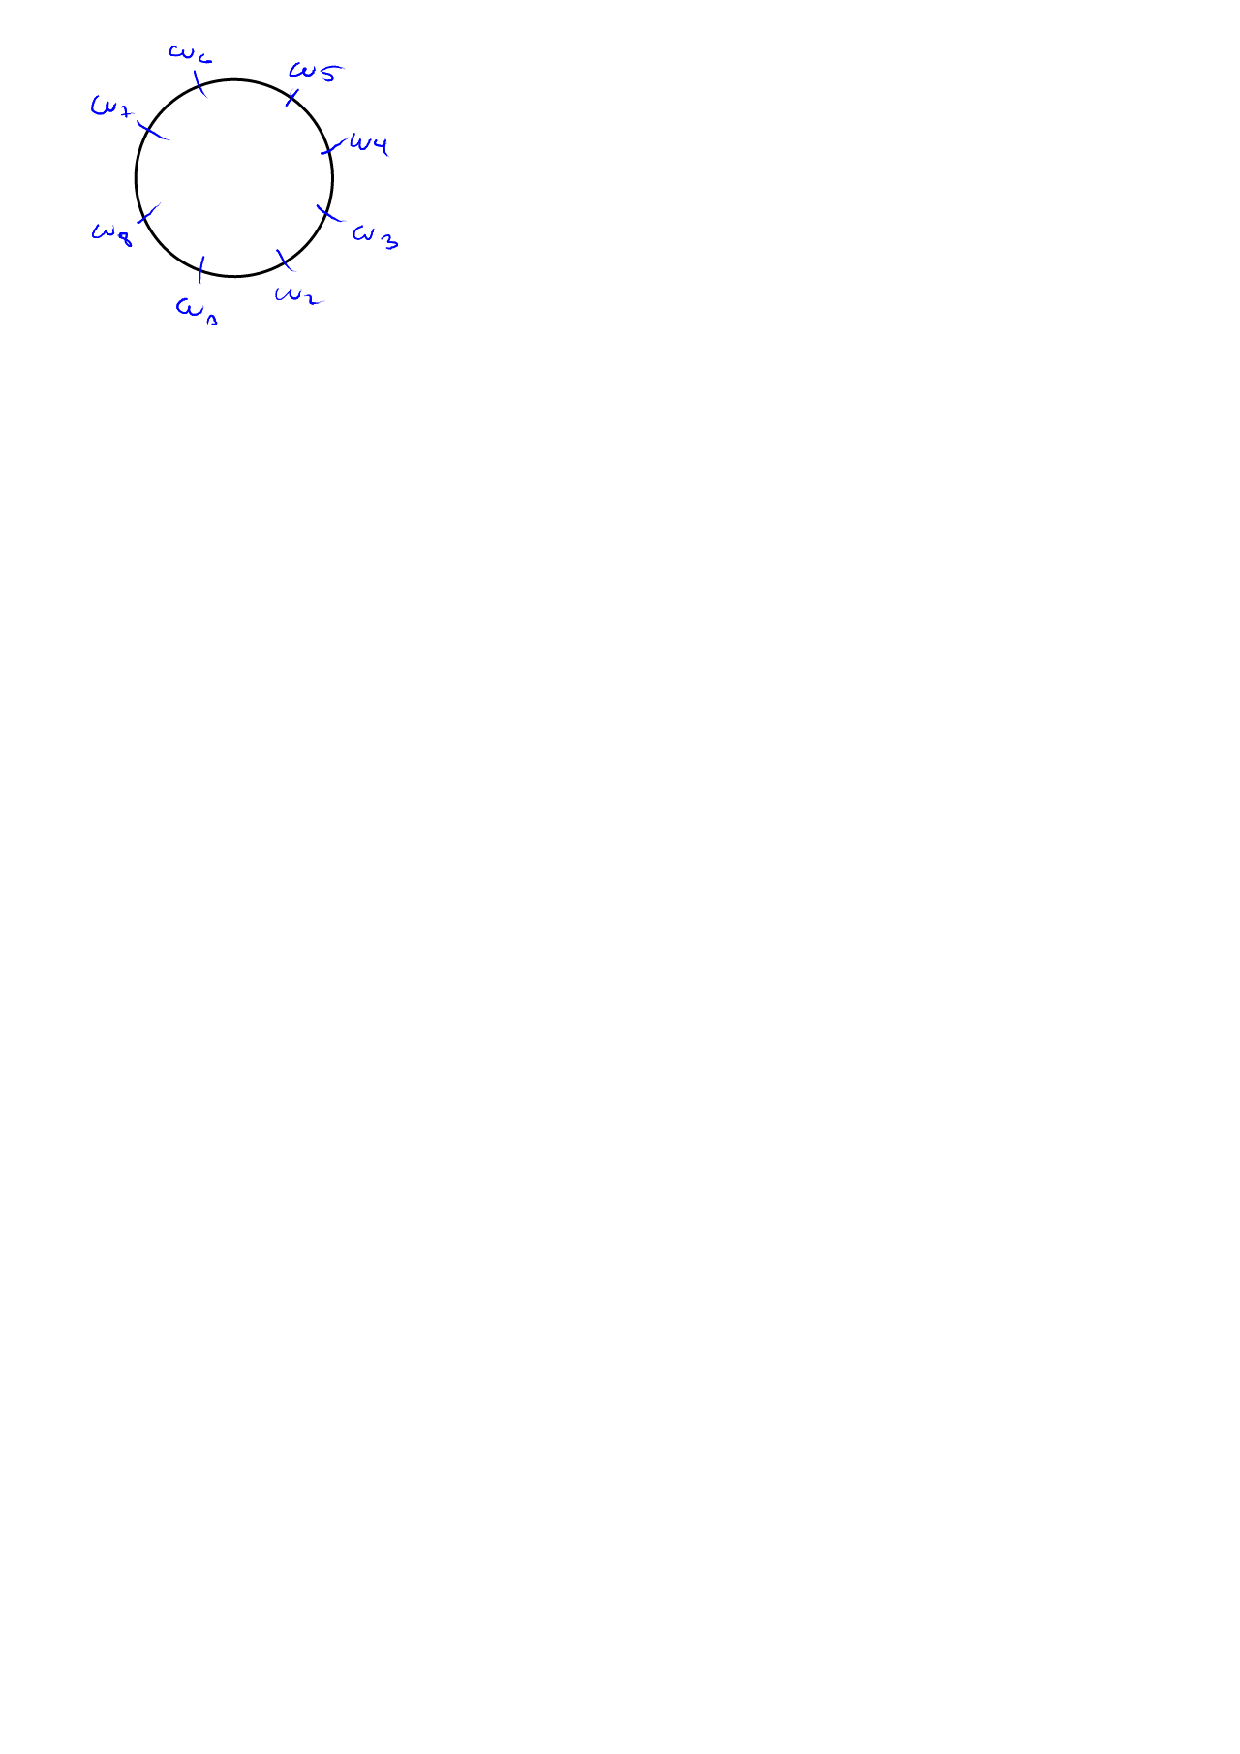
\includegraphics[trim=1.2cm 24cm 14cm .3cm]{\GraphicsFolder/kruh.pdf}
 \caption{Inserting fields on strings.}
 \label{Fig:GeomStr}
\end{figure}
We will be dealing with \emph{two ``dynamical'' theories:} one is the theory of fields $\omega\in \DR$ and one of field strings $\omega_1 \dotsb \omega_k \in \BCyc \DR$.

The field theory is at hand. We know that $(\DR,\Dd,\wedge,\langle\cdot,\cdot\rangle)$, where $\langle\omega_1,\omega_2\rangle = \int_M \omega_1 \wedge \omega_2$ for $\omega_1$, $\omega_2\in \DR$, is a \emph{symmetric dg-Frobenius algebra}. It is well-known that finite-dimensional Frobenius algebras $V$ are equivalent to $2$-dimensional topological quantum field theories (TQFT). Finite-dimensionality is a sufficient (and necessary) condition so that the trivial cylinder corresponding to the identity satisfies $\Id = \sum \langle \cdot,e^i\rangle e_i$. For now, we will ignore this issue and imagine $V=\DR$, although we will soon transfer to $\HDR$, where everything works just fine.
%One can also take the non-degenerate quotient of the small subalgebra of $\DR$ with respect to the canonical Hodge decomposition associated to a Riemannian metric on $M$. We denote it by $\VansQuotient(\VansSmall(\DR))$ and define in Chapter~\ref{Chap:5}. If our conjectures are correct, the results of our construction should be homotopy equivalent.
We will represent interactions of fields via Feynman graphs drawn on surfaces --- the trivial cylinder for fields, i.e., the free propagation, will be a line and the pair of pants, i.e., the interaction via the intersection $\wedge$, will be a point with $3$ segments emanating from it (we do not distinguish input and outputs by cyclic symmetry).

Let us now consider field strings. Figure \ref{Fig:OpCoOpDiag} defines the operations
\[ \OPQ_{210}: \hat{\Ext}_2 \DBCyc V \rightarrow \hat{\Ext}_1\DBCyc V \quad\text{and}\quad \OPQ_{120}: \hat{\Ext}_1\DBCyc V \rightarrow \hat{\Ext}_2\DBCyc V, \]
where $\Ext(\DBCyc V)$ is the exterior algebra canonically isomorphic to $\Sym(\DBCyc V [1])$. We read the diagram from the top to the bottom but imagine fields $\omega$ being fed into $\psi$'s from the bottom to the top. We think of these digrams as of \emph{string interaction diagrams} for strings freely moving in a topological space $M$, connecting and disconnecting.
\begin{figure}[t]
\centering
 %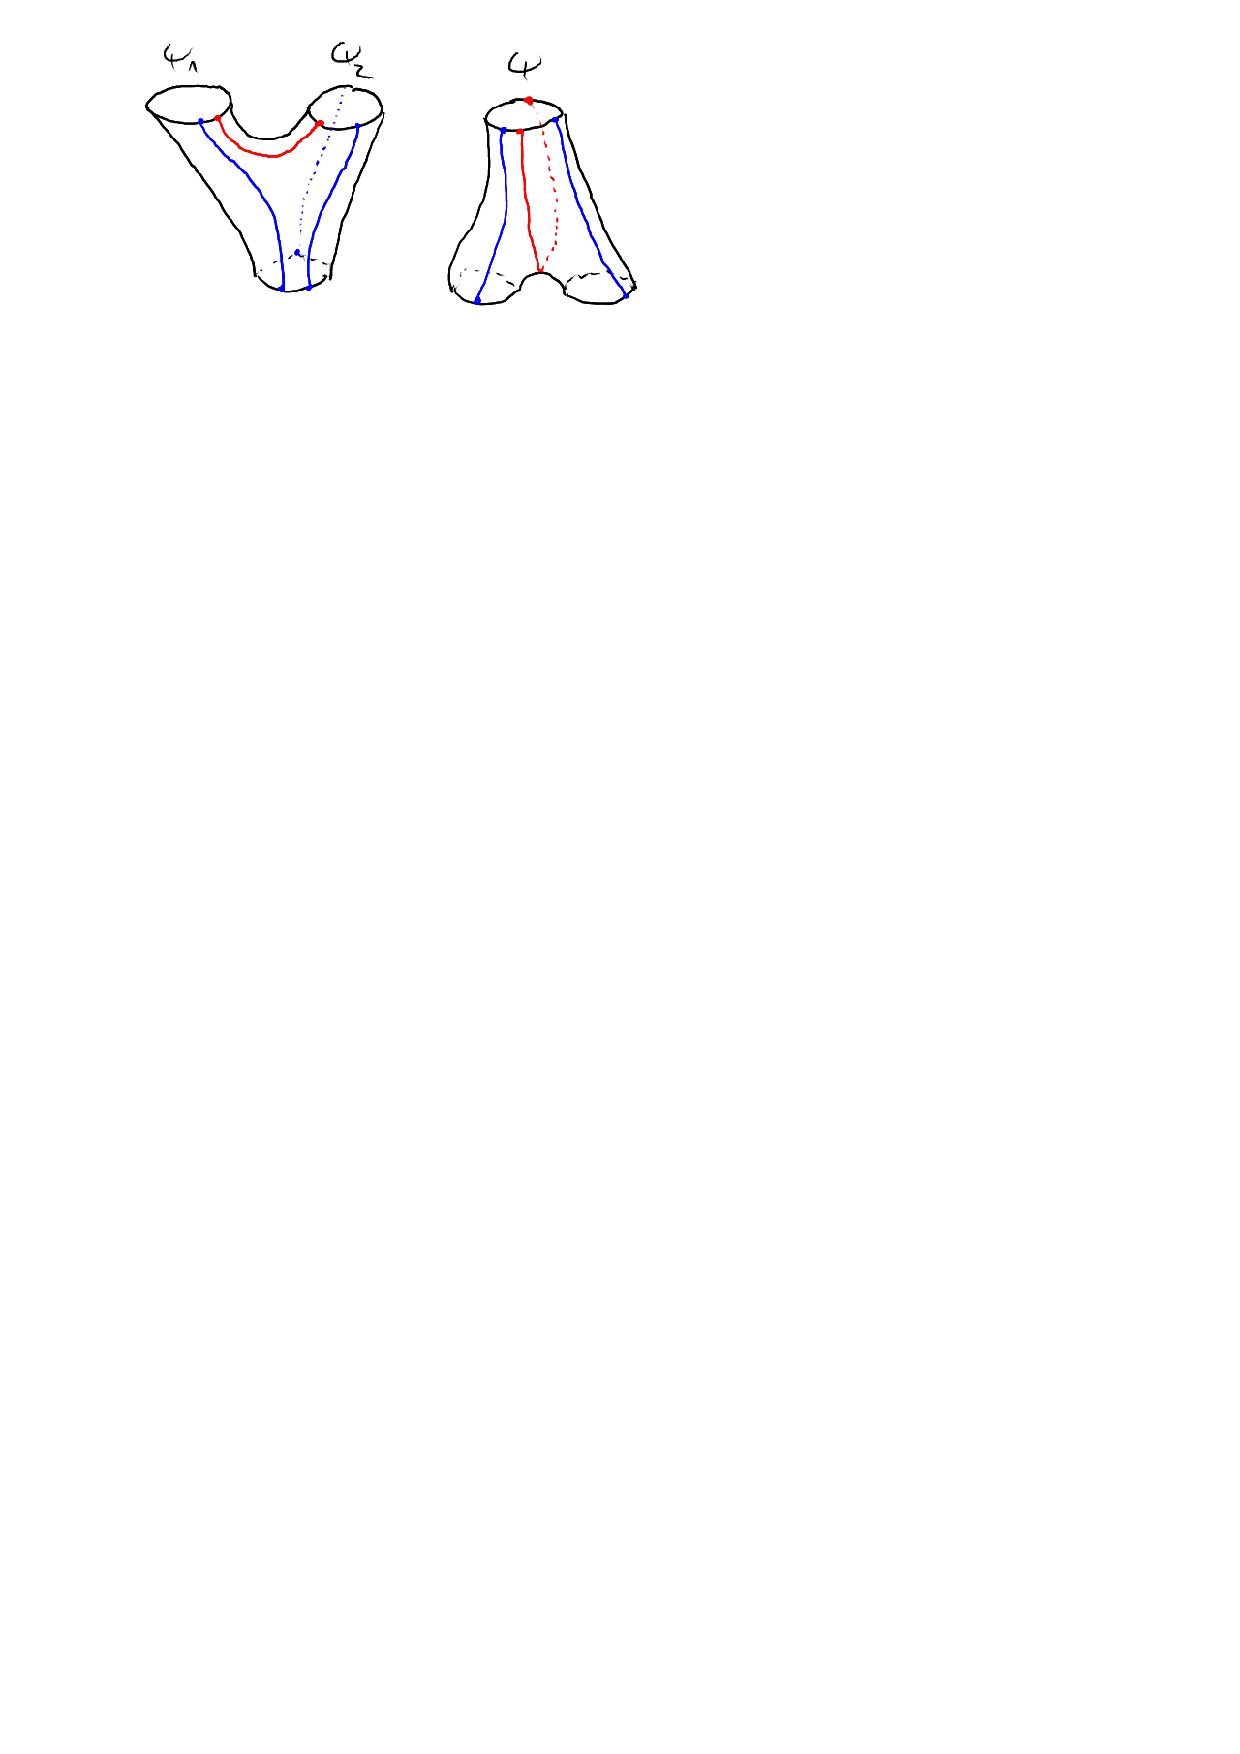
\includegraphics[trim=2cm 24cm 10cm .3cm]{\GraphicsFolder/op.pdf}
 \def\BddMin{.2}
\def\BddMaj{.4}
\def\HorLen{2}
\def\PMCVert{1}
\def\PantsVert{2}
\def\PantsPlunge{.5}
\newcommand{\BddSurf}[6][0]{
% #1 rotation (the optional argument)
% #2 is the center, e.g., C1 or 0:1
% #3 is the major semiaxis
% #4 is the minor semiaxis
% #5 is the style of the upper half
% #6 is the style of the lower half
\draw[#5,rotate=#1] ([shift=(0:{#3} and {#4})]#2) arc (0:180:{#3} and {#4});
\draw[#6,rotate=#1] ([shift=(180:{#3} and {#4})]#2) arc (180:360:{#3} and {#4});
%
}

\begin{tikzpicture}[scale=1.5]
\tikzset{point/.style = {draw, circle, fill=black, minimum size=2pt,inner sep=0pt}}
\coordinate (C1) at (0,0);
\coordinate (CC) at ($(C1) + (\HorLen,0)$);
\coordinate (CV) at ($(C1) + (.5*\HorLen,\PMCVert)$);

\coordinate (C2) at ($(CC) + (.5*\HorLen,-\PantsVert)$);
\coordinate (CP) at ($(CC) + (.5*\HorLen,-\PantsPlunge)$);
\coordinate (C3) at ($(CC) + (\HorLen,0)$);
 
\BddSurf{C2}{\BddMaj}{\BddMin}{dotted}{}
\BddSurf{C3}{\BddMaj}{\BddMin}{}{}
\BddSurf{CC}{\BddMaj}{\BddMin}{}{}

\draw ([shift={(-\BddMaj,0)}]CC) to[out=-90,in=90] ([shift={(-\BddMaj,0)}]C2);
\draw ([shift={(\BddMaj,0)}]C2) to[out=90,in=-90] ([shift={(\BddMaj,0)}]C3);

\draw ([shift={(\BddMaj,0)}]CC) to[out=-90,in=180] (CP);
\draw (CP) to[out=0,in=-90] ([shift={(-\BddMaj,0)}]C3);

\draw[thick,red]
 ([shift=(-40:{\BddMaj} and {\BddMin})]CC) to[out=-85,in=180]
([shift={(0,.-.25*\PantsPlunge)}]CP) to[out=0,in=-90] ([shift=(-140:{\BddMaj} and {\BddMin})]C3);

\draw ([shift=(245:{\BddMaj} and {\BddMin})]C2) to[out=90,in=-80] ([shift=(240:{\BddMaj} and {\BddMin})]CC);

\node[point,style={fill=white}] at ([shift=(245:{\BddMaj} and {\BddMin})]C2) {};
\node[point,style={fill=white}] at ([shift=(240:{\BddMaj} and {\BddMin})]CC) {};
\node[point,style={fill=white}] at ([shift=(-140:{\BddMaj} and {\BddMin})]C3) {};
\node[point,style={fill=white}] at ([shift=(-40:{\BddMaj} and {\BddMin})]CC) {};

\draw[dashed] ([shift=(110:{\BddMaj} and {\BddMin})]C2) to[out=90, in=-85] ([shift=(90:{\BddMaj} and {\BddMin})]CC);

\draw ([shift=(-60:{\BddMaj} and {\BddMin})]C2) to[out=90, in=-110] ([shift=(-40:{\BddMaj} and {\BddMin})]C3);

\draw[dashed] ([shift=(70:{\BddMaj} and {\BddMin})]C2) to[out=90, in=-90] ([shift=(80:{\BddMaj} and {\BddMin})]C3);

\node[label={[yshift=-.85cm] $\color{red}\mathrm{T}$}] at (CP) {};


\node[point,style={fill=white}] at ([shift=(80:{\BddMaj} and {\BddMin})]C3) {};
\node[point,style={fill=white}] at ([shift=(70:{\BddMaj} and {\BddMin})]C2) {};
\node[point,style={fill=white}] at ([shift=(-40:{\BddMaj} and {\BddMin})]C3) {};
\node[point,style={fill=white}] at ([shift=(-60:{\BddMaj} and {\BddMin})]C2) {};
\node[point,style={fill=white}] at ([shift=(90:{\BddMaj} and {\BddMin})]CC) {};
\node[point,style={fill=white}] at ([shift=(110:{\BddMaj} and {\BddMin})]C2) {};

\end{tikzpicture}
\quad\quad
\begin{tikzpicture}[scale=1.5]
\tikzset{point/.style = {draw, circle, fill=black, minimum size=2pt,inner sep=0pt}}
\coordinate (C1) at (0,0);
\coordinate (CC) at ($(C1) + (\HorLen,0)$);
\coordinate (C2) at ($(CC) + (.5*\HorLen,\PantsVert)$);
\coordinate (CP) at ($(CC) + (.5*\HorLen,\PantsPlunge)$);
\coordinate (C3) at ($(CC) + (\HorLen,0)$);
 
\BddSurf{C2}{\BddMaj}{\BddMin}{}{}
\BddSurf{C3}{\BddMaj}{\BddMin}{}{}
\BddSurf{CC}{\BddMaj}{\BddMin}{}{}

%Contour
\draw ([shift={(-\BddMaj,0)}]CC) to[out=90,in=-90] ([shift={(-\BddMaj,0)}]C2);
\draw ([shift={(\BddMaj,0)}]C2) to[out=-90,in=90] ([shift={(\BddMaj,0)}]C3);

\draw ([shift={(\BddMaj,0)}]CC) to[out=90,in=-180] (CP);
\draw (CP) to[out=0,in=90] ([shift={(-\BddMaj,0)}]C3);

%\draw[thick]([shift=(-40:{\BddMaj} and {\BddMin})]CC) to[out=85,in=-180]([shift={(0,.-.25*\PantsPlunge)}]CP) to[out=0,in=90] ([shift=(-140:{\BddMaj} and {\BddMin})]C3);

% Lines

\draw ([shift=(260:{\BddMaj} and {\BddMin})]C2) to[out=-90,in=90] ([shift=(280:{\BddMaj} and {\BddMin})]CC);

\draw ([shift=(210:{\BddMaj} and {\BddMin})]C2) to[out=-90, in=90] ([shift=(210:{\BddMaj} and {\BddMin})]CC);

\draw ([shift=(-30:{\BddMaj} and {\BddMin})]C2) to[out=-90, in=90] ([shift=(-50:{\BddMaj} and {\BddMin})]C3);

\draw[dashed] ([shift=(90:{\BddMaj} and {\BddMin})]C2) to[out=-90, in=90] ([shift=(140:{\BddMaj} and {\BddMin})]C3);

\node[point,style={fill=white}] at ([shift=(280:{\BddMaj} and {\BddMin})]CC) {};
\node[point,style={fill=white}] at ([shift=(210:{\BddMaj} and {\BddMin})]CC) {};

\node[point,style={fill=white}] at ([shift=(-30:{\BddMaj} and {\BddMin})]C2) {};
\node[point,style={fill=white}] at ([shift=(90:{\BddMaj} and {\BddMin})]C2)  {};
\node[point,style={fill=white}] at ([shift=(140:{\BddMaj} and {\BddMin})]C3) {};
\node[point,style={fill=white}] at ([shift=(-50:{\BddMaj} and {\BddMin})]C3) {};
\node[point,style={fill=white}] at ([shift=(210:{\BddMaj} and {\BddMin})]C2) {};
\node[point,style={fill=white}] at ([shift=(260:{\BddMaj} and {\BddMin})]C2) {};

\draw[red,thick,dashed] ([shift=(120:{\BddMaj} and {\BddMin})]C2) to[out=-90, in=120] (CP);
\draw[red,thick] ([shift=(-60:{\BddMaj} and {\BddMin})]C2) to[out=-90, in=60] (CP);

\node[point,style={fill=white}] at ([shift=(-60:{\BddMaj} and {\BddMin})]C2) {};
\node[point,style={fill=white}] at ([shift=(120:{\BddMaj} and {\BddMin})]C2) {};

\node[label={[yshift=-.7cm] $\color{red}\mathrm{T}$}] at (CP) {};
%\node[label={[yshift=-.7cm] $\scriptstyle \mathrm{T}$}] at (CP) {};
\end{tikzpicture}
 \caption[Operations $\OPQ_{210}$ and $\OPQ_{120}$.]{Operations $\OPQ_{210}$ and $\OPQ_{120}$. Fields propagate from the bottom to the top and an additional dualization, equivalently contraction with the identity propagator, is required when two outputs are connected; hence the red color.}
 \label{Fig:OpCoOpDiag}
\end{figure}
%$I^*(\sigma)$ localizes which 
%The output string will be localized at any field string which arose by propagating the focalized string fields along the diagram. I.e. on those which are obtained by propagating those on which the input strings are non-zero along the diagram.
%
%From the point of view of the TQFT, these propagators are trivial cylinders, and hence nothing is happening. 
This suggests that $\OPQ_{210}$ and $\OPQ_{120}$ are related to $\StringOp_2$ and $\StringCoOp_2$, respectively. Formulas for~$\OPQ_{210}$ and~$\OPQ_{120}$ for a finite dimensional symmetric dg-Frobenius algebra $V$ were written down in \cite{Cieliebak2015} and it was proven that they indeed constitute an $\IBL$-algebra on~$\DBCyc V$ (note that this is not a TQFT!). \ToDo[noline,caption={Which degree shift}]{Need to sort out which degree shift for bislgebra one needs! How is it with $2-n$.}As for the formulas, one simply decorates the world-lines of fields with the identity propagator $T = \sum_i e^i \otimes e_i$ and evaluates. As a mathematical remark, we will show that $\OPQ_{210}$ is obtained from the Gerstenhaber bracket on Hochschild cochains via cyclization by $\langle\cdot,\cdot\rangle$ and that $\OPQ_{120}$  is a factorization of an extension of the canonical Schwarz's $\BV$-operator on $\Fun(V[1])$ (odd degree shift of a finite-dimensional symmetric dg-Frobenius algebra is an odd symplectic vector space) to cyclic invariants with respect to the cyclic shuffle product.

Since $\DBCyc V [1]$ is not naturally an odd symplectic vector space, there is no Schwarz's $\BV$-operator on $\Fun(\DBCyc V [1])$. However, the following canonical operator
\[ \BVOp_{\mathrm{s}} \coloneqq  \hat{\OPQ}_{120} + \hbar \hat{\OPQ}_{210}: \Fun(\DBCyc V [1]) \rightarrow \Fun(\DBCyc V [1]), \]
where $\hat{\cdot}$ denote canonical extension to (co)derivatives, is a $\BV$-operator with respect to the function multiplication; we call it the \emph{string $\BV$-operator.} Recall that in physics, a $\BV$-operator $\BVOp$ on $\Fun(U)$, where $U$ is the space of fields,  is related to the measure in the path integral $\int_U \mu$. An action $S\in \Fun(U)$ satisfying the \emph{quantum master equation} (QME)
\[ \BVOp S + \frac{1}{2}\{S,S\} = 0 \]
defines a new measure $e^{-S} \mu$, and the corresponding twisted $\BV$-operator (or rather $\BVInfty$-operator) satisfies $\BVOp^S = e^{-S} \BVOp e^{S}$. For field strings, we define the following \emph{actions} $S_{\mathrm{free}}$, $S_{\mathrm{int}}\in \Fun(\BCyc V[1])$, which remind us of the \emph{Chern-Simons functional:}
\[S_{\mathrm{free}}(\omega_1 \omega_2) \coloneqq \pm \hbar^{-1}\int_M \omega_1 \wedge \Dd \omega_2 \quad\text{and}\quad S_{\mathrm{int}}(\omega_1 \omega_2 \omega_3) \coloneqq \pm \hbar^{-1}\int_M \omega_1 \wedge \omega_2 \wedge \omega_3.
\]
Note that $S_{\mathrm{free}}$ and $S_{\mathrm{int}}$ are linear functions on $\BCyc V[1]$ which vanish everywhere but field strings of lengths $2$ and $3$, respectively. It turns out that $S_{\mathrm{free}}$ and $S\coloneqq S_{\mathrm{free}} + S_{\mathrm{int}}$ satisfy the QME for $\BVOp_{s}$. The twisted $\BV$-operators look like
\[ \BVOp^{S_{\mathrm{free}}}_{s} = \hat{\OPQ}_{110} + \BVOp_{\mathrm{s}} \quad \text{and}\quad \BVOp^{S}_{s} = \hat{\OPQ}_{110} + \reallywidehat{\OPQ_{210}(S_{\mathrm{int}},\cdot)} + \BVOp_{\mathrm{s}}. \]
Figure~\ref{Fig:NewTerm} depicts the new terms $\OPQ_{110}$ and $\OPQ_{210}(S_{\mathrm{int}},\cdot)$ in $\BVOp^\Action_s$.
\begin{figure}[t]
 \centering
 \def\caphght{.6}
\def\BddMin{.2}
\def\BddMaj{.4}
\def\HorLen{2}
\def\PMCVert{1}
\def\PantsVert{2}
\def\PantsPlunge{.5}
\newcommand{\BddSurf}[6][0]{
% #1 rotation (the optional argument)
% #2 is the center, e.g., C1 or 0:1
% #3 is the major semiaxis
% #4 is the minor semiaxis
% #5 is the style of the upper half
% #6 is the style of the lower half
\draw[#5,rotate=#1] ([shift=(0:{#3} and {#4})]#2) arc (0:180:{#3} and {#4});
\draw[#6,rotate=#1] ([shift=(180:{#3} and {#4})]#2) arc (180:360:{#3} and {#4});
%
}
\vcenterline{
\begin{tikzpicture}[scale=1.5]
\tikzset{point/.style = {draw, circle, fill=black, minimum size=2pt,inner sep=0pt}}
\node at (0,.9) {};
\coordinate (CT) at (0,0);
\coordinate (CB) at (0,-\PantsVert);
\draw ([shift={(-\BddMaj,0)}]CB) -- ([shift={(-\BddMaj,0)}]CT);
\draw ([shift={(\BddMaj,0)}]CB) -- ([shift={(\BddMaj,0)}]CT);
\BddSurf{CB}{\BddMaj}{\BddMin}{dotted}{}
\BddSurf{CT}{\BddMaj}{\BddMin}{}{}
\node[point,style={fill=white}] (NT1) at ([shift=(-40:{\BddMaj} and {\BddMin})]CT) {};
\node[point,style={fill=white}] (NT2) at ([shift=(-100:{\BddMaj} and {\BddMin})]CT) {};
\node[point,style={fill=white}] (NT3) at ([shift=(140:{\BddMaj} and {\BddMin})]CT) {};
\node[point,style={fill=white}] (NT4) at ([shift=(70:{\BddMaj} and {\BddMin})]CT) {};
\node[point,style={fill=white}] (NB1) at ([shift=(-40:{\BddMaj} and {\BddMin})]CB) {};
\node[point,style={fill=white}] (NB2) at ([shift=(-100:{\BddMaj} and {\BddMin})]CB) {};
\node[point,style={fill=white}] (NB3) at ([shift=(140:{\BddMaj} and {\BddMin})]CB) {};
\node[point,style={fill=white}] (NB4) at ([shift=(70:{\BddMaj} and {\BddMin})]CB) {};
\draw (NT1) -- (NB1);
\draw (NT2) -- (NB2);
\draw[dashed] (NT3) -- (NB3);
\draw[dashed] (NT4) -- (NB4);
\node[fill=white] at ($.5*(NT2)+.5*(NB2)$) {$\color{green}\Dd$};
\end{tikzpicture}}
\qquad + \qquad\vcenterline{
\begin{tikzpicture}[scale=1.5]
\tikzset{point/.style = {draw, circle, fill=black, minimum size=2pt,inner sep=0pt}}
\coordinate (C1) at (0,0); % left most
\coordinate (CC) at ($(C1) + (\HorLen,0)$); % the connection
\coordinate (CV) at ($(C1) + (.5*\HorLen,\PMCVert)$); % the vertical one

\coordinate (C2) at ($(CC) + (.5*\HorLen,-\PantsVert)$); % the right bottom one
\coordinate (CP) at ($(CC) + (.5*\HorLen,-\PantsPlunge)$); % the middle of propagator
\coordinate (C3) at ($(CC) + (\HorLen,0)$); % the right one

\coordinate (CT) at ($(CC) + (0,\caphght)$);
\draw ($(CC) + (-\BddMaj,0)$) to[out=90,in=180] (CT);
\draw (CT) to[out=0,in=90] ($(CC)+(\BddMaj,0)$);

\BddSurf{C2}{\BddMaj}{\BddMin}{dotted}{}
\BddSurf{C3}{\BddMaj}{\BddMin}{}{}
\BddSurf{CC}{\BddMaj}{\BddMin}{dotted}{dotted}

\draw ([shift={(-\BddMaj,0)}]CC) to[out=-90,in=90] ([shift={(-\BddMaj,0)}]C2);
\draw ([shift={(\BddMaj,0)}]C2) to[out=90,in=-90] ([shift={(\BddMaj,0)}]C3);

\draw ([shift={(\BddMaj,0)}]CC) to[out=-90,in=180] (CP);
\draw (CP) to[out=0,in=-90] ([shift={(-\BddMaj,0)}]C3);

\draw[thick,red] (CT) to[out=-50,in=90] ([shift=(-40:{\BddMaj} and {\BddMin})]CC) to[out=-85,in=180] ([shift={(0,.-.25*\PantsPlunge)}]CP) to[out=0,in=-90] ([shift=(-140:{\BddMaj} and {\BddMin})]C3);
% The identity line

%START: Inputs from C2
\draw ([shift=(245:{\BddMaj} and {\BddMin})]C2) to[out=90,in=-80] ([shift=(240:{\BddMaj} and {\BddMin})]CC) to[out=90,in=-120] (CT);

\draw[dashed] ([shift=(110:{\BddMaj} and {\BddMin})]C2) to[out=90, in=-85] ([shift=(90:{\BddMaj} and {\BddMin})]CC) to[out=90,in=-90] (CT);


\draw ([shift=(-60:{\BddMaj} and {\BddMin})]C2) to[out=90, in=-110] ([shift=(-40:{\BddMaj} and {\BddMin})]C3);

\draw[dashed] ([shift=(70:{\BddMaj} and {\BddMin})]C2) to[out=90, in=-90] ([shift=(80:{\BddMaj} and {\BddMin})]C3);
%END: Inputs from C2


%\node[label={[yshift=.1cm] $\psi$}] at (C3) {};
\node[label={[yshift=-.8cm] $\color{red}\mathrm{T}$}] at (CP) {};

\node[point,style={fill=white}] at ([shift=(80:{\BddMaj} and {\BddMin})]C3) {};

\node[point,style={fill=white}] at ([shift=(-40:{\BddMaj} and {\BddMin})]C3) {};

\node[point,style={fill=white}] at ([shift=(-140:{\BddMaj} and {\BddMin})]C3) {};
\node[point,style={fill=white}] at ([shift=(245:{\BddMaj} and {\BddMin})]C2) {};
\node[point,style={fill=white}] at ([shift=(110:{\BddMaj} and {\BddMin})]C2) {};
\node[point,style={fill=white}] at ([shift=(-60:{\BddMaj} and {\BddMin})]C2) {};
\node[point,style={fill=white}] at ([shift=(70:{\BddMaj} and {\BddMin})]C2) {};

\node[point,label={[above]$\color{green}\wedge$}] at (CT) {};

\end{tikzpicture}}
 %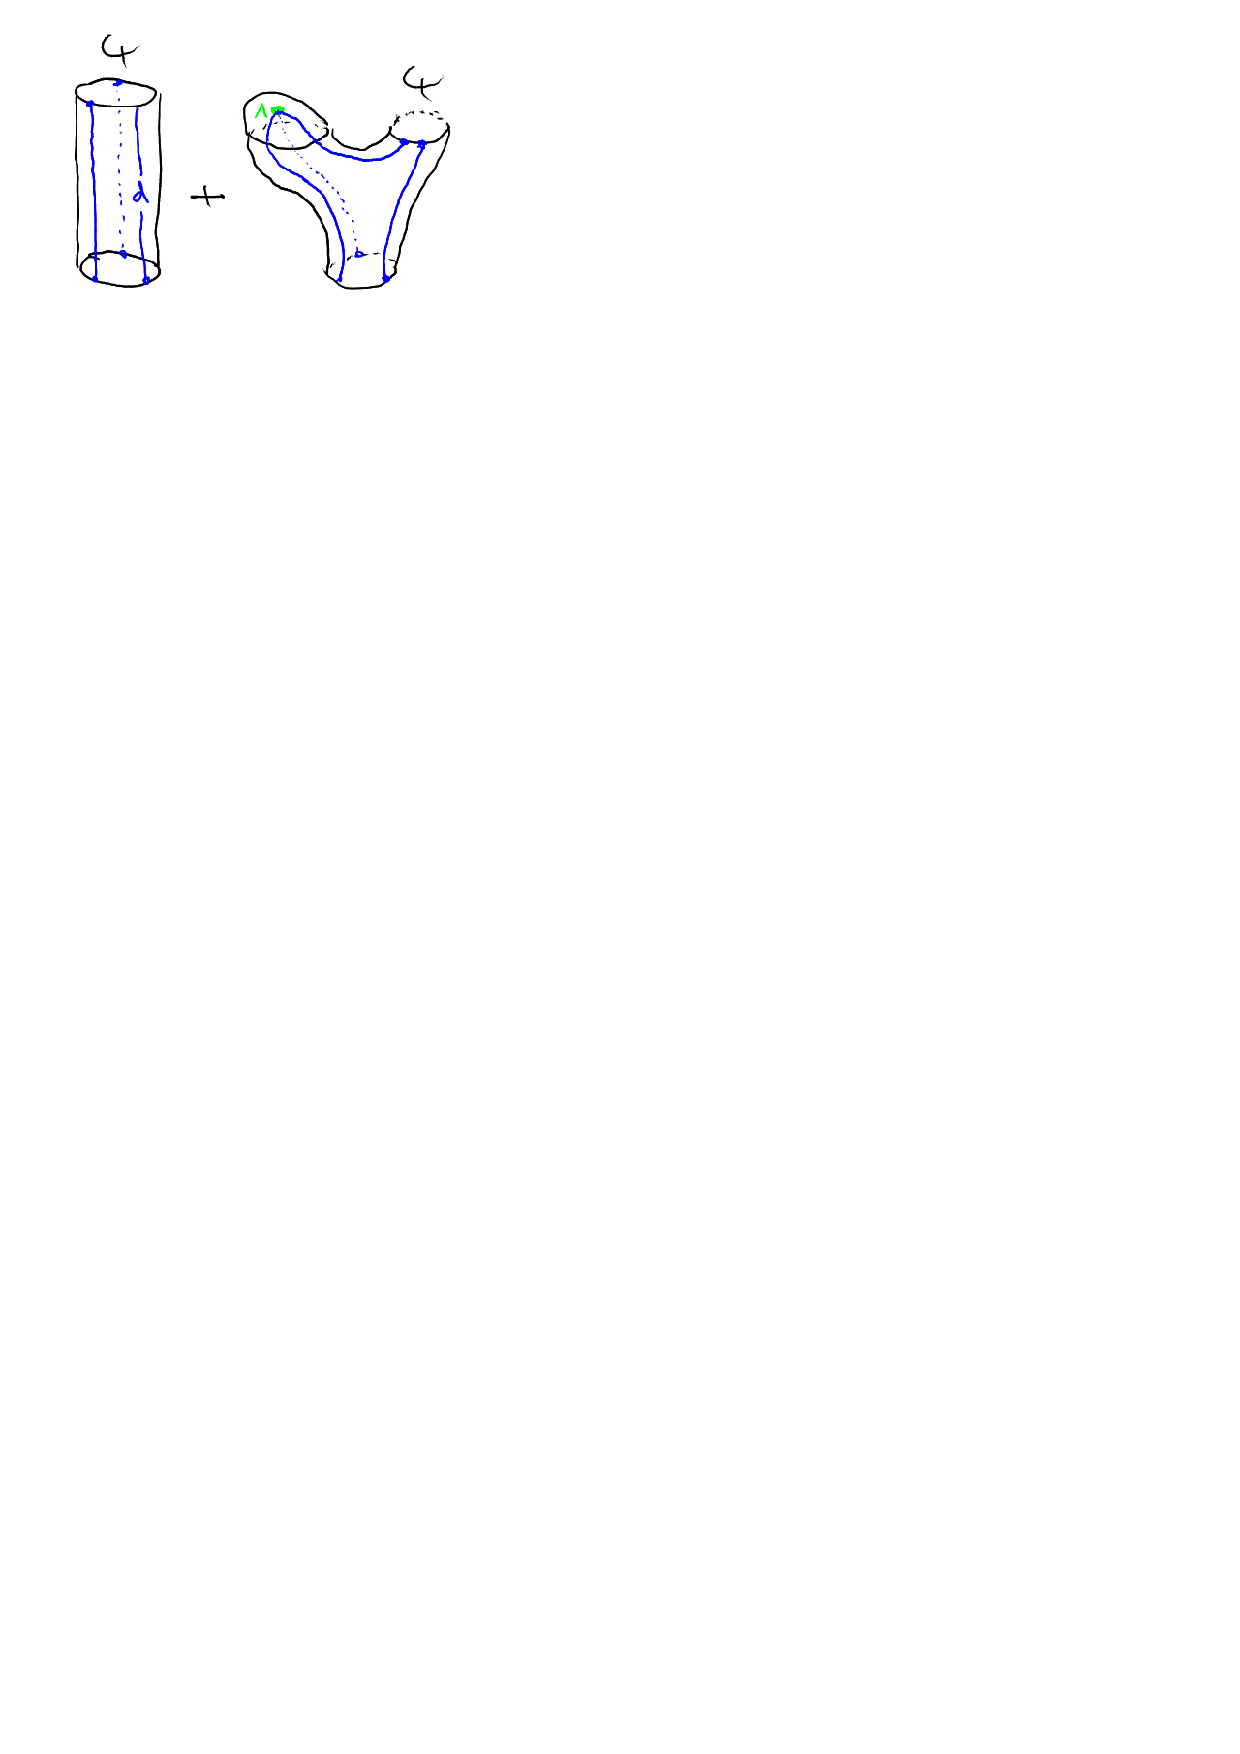
\includegraphics[trim=1cm 24.5cm 12.6cm .4cm]{\GraphicsFolder/diff.pdf}
 \caption{Adding $\Dd$ and $\wedge$ via $\Action$.}
 \label{Fig:NewTerm}
\end{figure}
The corresponding $\dIBL$-algebra reads
\[ \Bigl(\DBCyc V,\OPQ_{110}^\MC\coloneqq \OPQ_{110} + \OPQ_{210}(S_{\mathrm{int}},\cdot),\OPQ_{210},\OPQ_{120}\Bigr), \]
where we recognize the Hochschild differential $\OPQ_{110}^\MC$. If this was well-defined for $V = \DR$, then it would give the $\IBLInfty$-chain model of string topology.

%They are all define $\dIBL$-structures on $\DR$ then 
%$\Model \coloneqq \CycC(\DR)$ with the $\dIBL$-structure $(\OPQ_{110} + \OPQ_{210}(S_{\text{free}},\cdot), \OPQ_{210}, \OPQ_{120})$ would be the correct $\IBLInfty$-chain model for string topology.  
%Making from operations $V^{\otimes k} \rightarrow V$ is called cyclization and we normaly non-degenerate pairing for that.

As in quantum field theories, we are going to ``formally'' \emph{integrate out redundant degrees of freedom in the path integral} of our ill-defined theory and obtain a well-defined theory on $\DBCyc\HDR$, which is ``formally'' homotopy equivalent to the original one. We pick a Riemannian metric on $M$ and consider the Hodge decomposition $\DR = \Harm \oplus \Im\Dd \oplus \Im\CoDd$, where $\Harm \simeq \HDR$ are the harmonic forms $\Dd \omega = \CoDd \omega = 0$. For Chern-Simons fields $\omega\in \DR$, one thinks of $\Dd \omega = 0$ as of the Euler-Lagrange equation and of $\CoDd \omega = 0$ as of the Lorentz gauge. The ``inverse'' of $\Dd$ as a map $\Im\Dd \rightarrow \Im \CoDd$ is the standard Hodge homotopy $\HtpStd$, i.e., the unique coexact solution of $\Dd \Htp + \Htp \Dd = \Id - \pi_\Harm$, were $\pi_\Harm: \DR \rightarrow \Harm$ is the orthogonal projection. The Schwartz kernel of $\HtpStd$ is the \emph{standard Hodge propagator} $\PrpgStd$. A formula for the \emph{effective action} $W\in\Fun(\BCyc\HDR[1])$ was given in \cite{Cieliebak2015}; in their terminology, it would be called the \emph{(formal) pushforward Maurer-Cartan element}. We have
\[ W = \hbar^{-1}\sum_{l\ge 1, g\ge 0} \PMC_{lg} \hbar^{g}, \]
where $\PMC_{lg} \in \hat{\Ext}_l \DBCyc\HDR$ is computed from $(l+g-1)$-loop Feynman diagrams with interaction vertices $\wedge$ and propagator $\StdPrpg$. One can think of trying to push the field strings to their representatives consisting of harmonic forms. The twisted string $\BV$-operator on $\Fun(\BCyc\HDR[1])$ reads
\[ \BVOp^W_s = \hat{\OPQ}^{\PMC}_{110}  +  \hbar{\OPQ}_{210} + \sum_{l\ge 2, g\ge 0} \hat{\OPQ}^{\PMC}_{1lg} \hbar^{g}, \]
where $\OPQ_{110}^\PMC = \OPQ_{210}(\PMC_{10},\cdot) = \OPQ_{210}\circ_1 \PMC_{10}$ and $\OPQ_{1lg}^\PMC = \OPQ_{210}\circ \PMC_{lg}$. The resulting $\IBLInfty$-structure on $\CDBCyc\HDR$, i.e., our chain model of equivariant string topology, is, in fact, a \emph{quantum $\CoLInfty$-algebra $(\OPQ_{1lg}^\PMC)$ with Drinfeld-compatible Lie bracket $\OPQ_{210}$.} The weak homotopy equivalence of $(\CDBCyc\HDR,\OPQ_{110}^\PMC)$ and $(C(\StringSpace M),\Bdd)$ inducing an isomorphism of the $\IBL$-structure on homology is given by the composition $F\circ I^*: C(\StringSpace M) \rightarrow \CDBCyc \HDR$, where 
\[ F = \HTP_{110} + \HTP_{210}\circ_1 \MC_{10} + \frac{1}{2!} \HTP_{310}\circ_{1,1}(\MC_{10},\MC_{10}) + \dotsb \]
with $\HTP_{110} = \iota^*$ for $\iota: \HDR\simeq \Harm \xhookrightarrow{} \DR$, and where $\HTP_{k10}\circ_{1,\dotsc,1}(\MC_{10},\dotsc,\MC_{10})$ contributes by trivalent trees as in Figure~\ref{Fig:KSTree}.
\begin{figure}[t]
\centering
\[\underbrace{\vcenterline{\begin{tikzpicture}[scale=1,
every label/.append style={font=\scriptsize},
point/.style = {draw, circle, fill=black, minimum size=2pt,inner sep=0pt},
leaf/.style = {draw, circle, fill=white, minimum size=2pt,inner sep=0pt},
]
\def\vertdist{.8}
\def\hordist{.6}
\node[leaf] (R) at (0,0) {};
\node[point, label={[right,yshift=-1mm] $\color{green}\wedge$}] (RU) at ($(R) + (0,\vertdist)$) {};
\node[point, label={[right] $\color{green}\wedge$}] (RUL) at ($(RU) + (-2*\hordist,\vertdist)$) {};
\node[point, label={[right] $\color{green}\wedge$}] (RUR) at ($(RU) + (2*\hordist,\vertdist)$) {};
\node[point, label={[right] $\color{green}\wedge$}] (RULL) at ($(RUL) + (-1*\hordist,1*\vertdist)$) {};
\coordinate (RULR) at ($(RUL) + (\hordist,\vertdist)$);
\coordinate (RURR) at ($(RUR) + (\hordist,\vertdist)$);
\node[leaf, label={[right] $h_1$}] (RULLL) at ($(RULL) + (-1*\hordist,1*\vertdist)$){};
\node[leaf, label={[right] $h_2$}] (RULLR) at ($(RULL) + (1*\hordist,1*\vertdist)$) {};
\node[leaf, label={[right] $h_3$}] (RULRR) at ($(RULR) + (1*\hordist,1*\vertdist)$) {};
\node[leaf, label={[right] $h_k$}] (RURRR) at ($(RURR) + (1*\hordist,1*\vertdist)$) {};
\node[] (RURRL) at ($(RURR) + (-1*\hordist,1*\vertdist)$) {\ \,\dots};
\node (RURL) at ($(RUR) + (-\hordist,\vertdist)$) {\dots};
\draw (R) edge (RU); 
\draw[thick,blue] (RU) -- (RUL) node[below,midway,shift={(-2mm,1mm)}] {$\Htp$}; 
\draw[thick,blue] (RUL) -- (RULL) node[below,midway,shift={(-2mm,1.5mm)}] {$\Htp$}; 
\draw (RULL) edge (RULLL);
\draw (RULL) edge (RULLR);
\draw (RUL) edge (RULRR);
\draw[thick,blue] (RU) -- (RUR) node[below,midway,shift={(2mm,1mm)}] {$\Htp$};
\draw[thick,blue] (RUR) edge (RURL);
\draw (RUR) edge (RURRR);
\end{tikzpicture}}}_{\begin{multlined} \wedge \circ (\Htp \otimes \Htp)\circ (\wedge \otimes \wedge)\circ (\Htp \otimes \Id \otimes \dotsb  \otimes \Id)\\
 \circ (\wedge \otimes \Id \otimes \dotsb \otimes \Id)(h_1, h_2, h_3, \dots, h_k).
\end{multlined}}\]
\caption{Kontsevich-Soibelman evaluation of a decorated tree.}
\label{Fig:KSTree}
\end{figure}
Note that in order to evaluate trees, we do not need the Schwartz kernel $\Prpg$ and hence any pairing. The homotopy $\Htp$ is enough because the graph is directed and we can distinguish inputs and outputs. On the other hand, evaluation of the $1$-loop Feynman graph in Figure~\ref{Fig:OneLoopDiag} contributing to $\OPQ_{120}^\PMC$, for instance, requires $\Prpg$, and hence $\langle\cdot,\cdot\rangle$. From Sullivan's minimal model theory it is well-known that the homotopy type of the homotopy transfered $\AInfty$-structure $(\HDR,(m_k))$ is a topological invariant which encodes the rational homotopy theory of a simply-connected manifold $M$. Our construction can be seen as being associated to the Poincar\'e $\DGA$ $(\DR,\Dd,\wedge, \langle\cdot,\cdot\rangle)$, i.e, a $\DGA$ whose homology is a Poincar\'e duality algebra. It is not clear to the author what kind of invariant is the weak homotopy type of the Poincar\'e $\DGA$ and what kind of invariant is the homotopy type of the twisted $\IBLInfty$-algebra on $\CDBCyc \HDR$. However, if $M$ is formal in the sense of $\DGA$'s, then $M$ is formal in the sense of Poincar\'e $\DGA$'s, and we conjecture that it is formal also in the sense of $\IBLInfty$-algebras; i.e., the twisted $\IBLInfty$-algebra on $\CDBCyc \HDR$ is homotopy equivalent to the canonical $\IBL$-algebra.
\begin{figure}[t]
\centering
\def\BddMin{.2}
\def\BddMaj{.4}
\def\HorLen{2}
\def\PMCVert{1}
\def\PantsVert{2}
\def\PantsPlunge{.5}
\newcommand{\BddSurf}[6][0]{
% #1 rotation (the optional argument)
% #2 is the center, e.g., C1 or 0:1
% #3 is the major semiaxis
% #4 is the minor semiaxis
% #5 is the style of the upper half
% #6 is the style of the lower half
\draw[#5,rotate=#1] ([shift=(0:{#3} and {#4})]#2) arc (0:180:{#3} and {#4});
\draw[#6,rotate=#1] ([shift=(180:{#3} and {#4})]#2) arc (180:360:{#3} and {#4});
%
}
\begin{tikzpicture}[scale=1.5]
\tikzset{point/.style = {draw, circle, fill=black, minimum size=2pt,inner sep=0pt}}
\coordinate (C1) at (0,0);
\coordinate (CC) at ($(C1) + (\HorLen,0)$);
\coordinate (CV) at ($(C1) + (.5*\HorLen,\PMCVert)$);

\coordinate (C2) at ($(CC) + (.5*\HorLen,-\PantsVert)$);
\coordinate (CP) at ($(CC) + (.5*\HorLen,-\PantsPlunge)$);
\coordinate (C3) at ($(CC) + (\HorLen,0)$);
 
\BddSurf{C1}{\BddMaj}{\BddMin}{dotted}{}
\BddSurf{C2}{\BddMaj}{\BddMin}{dotted}{}
\BddSurf{C3}{\BddMaj}{\BddMin}{}{}
\BddSurf{CC}{\BddMaj}{\BddMin}{dotted}{dotted}

\draw ([shift={(\BddMaj,0)}]C1) to[out=90,in=180] ([shift={(0,-\BddMaj)}]CV);
\draw ([shift={(0,-\BddMaj)}]CV) to[out=0,in=90] ([shift={(-\BddMaj,0)}]CC);
\draw ([shift={(-\BddMaj,0)}]CC) to[out=-90,in=90] ([shift={(-\BddMaj,0)}]C2);
\draw ([shift={(\BddMaj,0)}]C2) to[out=90,in=-90] ([shift={(\BddMaj,0)}]C3);
% Lower countour

\draw ([shift={(-\BddMaj,0)}]C1) to[out=90,in=180] ([shift={(0,\BddMaj)}]CV);
\draw ([shift={(0,\BddMaj)}]CV) to[out=0,in=90] ([shift={(\BddMaj,0)}]CC);
\draw ([shift={(\BddMaj,0)}]CC) to[out=-90,in=180] (CP);
\draw (CP) to[out=0,in=-90] ([shift={(-\BddMaj,0)}]C3);
% Upper contour


\BddSurf[90]{CV}{\BddMaj}{\BddMin}{dashed,thick,blue}{thick,blue}
% The joint

\draw[red,thick] ([shift=(45:{\BddMin} and {\BddMaj})]CV) to[out=0,in=95] ([shift=(-40:{\BddMaj} and {\BddMin})]CC) to[out=-85,in=180] ([shift={(0,.-.25*\PantsPlunge)}]CP) to[out=0,in=-90] ([shift=(-140:{\BddMaj} and {\BddMin})]C3);
% The identity line


%START: Inputs from C1
\draw ([shift=(-60:{\BddMaj} and {\BddMin})]C1) to[out=90,in=180] ([shift=(-20:{\BddMin} and {\BddMaj})]CV);

\draw ([shift=(-110:{\BddMaj} and {\BddMin})]C1) to[out=90,in=180] ([shift=(20:{\BddMin} and {\BddMaj})]CV);

\draw[dashed] ([shift=(125:{\BddMaj} and {\BddMin})]C1) to[out=80,in=180] ([shift=(145:{\BddMin} and {\BddMaj})]CV);
%END: Inputs from C1

%START: Inputs from C2
\draw ([shift=(245:{\BddMaj} and {\BddMin})]C2) to[out=90,in=-80] ([shift=(240:{\BddMaj} and {\BddMin})]CC) to[out=100,in=0] ([shift=(-50:{\BddMin} and {\BddMaj})]CV);

\draw[dashed] ([shift=(110:{\BddMaj} and {\BddMin})]C2) to[out=90, in=-85] ([shift=(90:{\BddMaj} and {\BddMin})]CC) to[out=95, in=15] ([shift=(190:{\BddMin} and {\BddMaj})]CV);

\draw ([shift=(-60:{\BddMaj} and {\BddMin})]C2) to[out=90, in=-110] ([shift=(-40:{\BddMaj} and {\BddMin})]C3);

\draw[dashed] ([shift=(70:{\BddMaj} and {\BddMin})]C2) to[out=90, in=-90] ([shift=(80:{\BddMaj} and {\BddMin})]C3);
%END: Inputs from C2

\node[point,style={fill=white}] at ([shift=(-140:{\BddMaj} and {\BddMin})]C3) {};
\node[point] at ([shift=(190:{\BddMin} and {\BddMaj})]CV) {};

\node[point] at ([shift=(45:{\BddMin} and {\BddMaj})]CV) {};
\node[point] at ([shift=(-50:{\BddMin} and {\BddMaj})]CV) {};
\node[point] at([shift=(20:{\BddMin} and {\BddMaj})]CV) {};
\node[point] at ([shift=(-20:{\BddMin} and {\BddMaj})]CV) {};
\node[point] at ([shift=(145:{\BddMin} and {\BddMaj})]CV) {};

\node[label={[yshift=.2cm] $\psi$}] at (C3) {};
%\node[label={[yshift=-.9cm] $\omega_1$}] at (C1) {};
%\node[label={[yshift=-.9cm] $\omega_2$}] at (C2) {};
\node[label={[yshift=-.8cm] $\color{red}\mathrm{T}$}] at (CP) {};
\node at ([shift={(0,-\BddMin)}]CV) {};

% External labels at the first boundary component
\node[point,style={fill=white},label={[below,yshift=-.1cm,xshift=.1cm] $\scriptstyle h_{13}$}] at ([shift=(-60:{\BddMaj} and {\BddMin})]C1) {};
\node[point,style={fill=white},label={[below,yshift=-.1cm,xshift=-.1cm] $\scriptstyle h_{12}$}] at ([shift=(-110:{\BddMaj} and {\BddMin})]C1) {};
\node[point,style={fill=white},label={[below,yshift=+.1cm,xshift=-.6cm] $\scriptstyle h_{11}$}] at ([shift=(125:{\BddMaj} and {\BddMin})]C1) {};

% External labels at the second boundary component
\node[point,style={fill=white},label={[below,xshift=-.1cm,yshift=-.1cm] $\scriptstyle h_{22}$}] at ([shift=(245:{\BddMaj} and {\BddMin})]C2) {};
\node[point,style={fill=white},label={[left,xshift=-.4cm] $\scriptstyle h_{21}$}] at ([shift=(110:{\BddMaj} and {\BddMin})]C2) {};
\node[point,style={fill=white},label={[below,xshift=.1cm,yshift=-.1cm] $\scriptstyle h_{23}$}] at ([shift=(-60:{\BddMaj} and {\BddMin})]C2) {};
\node[point,style={fill=white},label={[right,xshift=.4cm] $\scriptstyle h_{24}$}] at ([shift=(70:{\BddMaj} and {\BddMin})]C2) {};


% Internal labels of vertices
\node[label={[above,yshift=.03cm] $\scriptstyle x_1$}] at ([shift=(145:{\BddMin} and {\BddMaj})]CV) {};
\node[label={[above,yshift=-.05cm,xshift=.1cm] $\scriptstyle x_2$}] at ([shift=(45:{\BddMin} and {\BddMaj})]CV) {};
\node[label={[right,xshift=-.04cm,yshift=-.18cm] $\scriptstyle x_3$}] at ([shift=(20:{\BddMin} and {\BddMaj})]CV) {};
\node[label={[right,yshift=-.25cm,xshift=-.05cm] $\scriptstyle x_4$}] at ([shift=(-20:{\BddMin} and {\BddMaj})]CV) {};
\node[label={[below,yshift=-.27cm] $\scriptstyle x_5$}] at ([shift=(-50:{\BddMin} and {\BddMaj})]CV) {};
\node[label={[left,yshift=-.24cm,xshift=.05cm] $\scriptstyle x_6$}] at ([shift=(190:{\BddMin} and {\BddMaj})]CV) {};
\node[font=\footnotesize] (ZZ) at ([shift={(0,-4.5ex)}]CV) {$\color{blue}\Prpg$};
\end{tikzpicture}
\[\begin{aligned}
=&\sum_{a,b}\sum_{c=1}^4 \pm  \mathrm{T}^{ab} \psi(e_a  h_{2,c+2}  h_{2,c+3})  \Bigl(\int_{x_1 x_2 x_3 x_4 x_5 x_6} \Prpg(x_1,x_2)\Prpg(x_2,x_3)\Prpg(x_3,x_4)\\
&\Prpg(x_4,x_5)\Prpg(x_5,x_6)\Prpg(x_6,x_1)\bigl( h_{11}(x_1) h_{12}(x_3)
h_{13}(x_4)\bigr)\bigl(e_b(x_2)  h_{2,c}(x_6)  h_{2,c+1}(x_5)\bigr)\Bigr)
\end{aligned}
\]
\caption{A $1$-loop diagram and its contribution to the twisted cobracket.}
\label{Fig:OneLoopDiag}
\end{figure}

Finally, note that from the theory of Koszul (pr)operads it is well-known that $\IBL$ is Koszul dual to $\Frob$, i.e., $\IBL^! = \Frob$ and $\Frob^! = \IBL$, where $\Frob$ is the properad of Frobenius bialgebras.
%(the coproduct is obtained from the product by dualization).
Therefore, it holds $\IBLInfty = \Omega(\Frob^*)$, where $\Omega$ denotes the cobar construction and ${}^*$ the linear dual coproperad; this precisely reflects our situation of having a Frobenius structure on $\HDR$ (the coproduct is obtained from the product via dualization) and $\IBLInfty$-structure on $\CDBCyc \HDR = \reallywidehat{\BCyc\HDR^*}$, where $\hat{\cdot}$ denotes a suitable completion, since $\BCyc$ is a cyclic version of the cobar construction.

\section{Relevant work of others}

In \cite{Cohen2001}, there is a homotopy theoretical realization of string topology operations $\StringOp_2$ and $\StringCoOp_2$. This is another approach to their rigorous definition.

In \cite{Cieliebak2007}, they sketch a proof that symplectic field theory of the unit cotangent bundle of $M$ and equivariant string topology of $M$ are $\IBLInfty$-quasi-isomorphic via a map induced from evaluations at boundaries of holomorphic curves. String topology operations then arise naturally from the structure of codimension $1$ boundary stratas of the moduli space of holomorphic curves with certain boundary conditions. In fact, a precise formulation of this correspondence was perhaps the main reason for Cieliebak \& Latschev to think about the $\IBLInfty$-chain model of string topology.\ToDo[caption={Precise formulation of SFT},noline]{How is it precisely, what kind of boundary conditions and punctures?}

An $\IBLInfty$-structure on the singular equivariant chain complex was proposed by \cite{Sullivan2005}. It is constructed using ``diffusion intersection product'' which realizes the intersection on the chain level. In fact, there is much more string operations coming from stacks of Sullivan diagrams than just the bracket and cobracket.

There is a recent construction of chain level non-equivariant string topology on the singular chain complex of $\Loop M$ using fat graphs \cite{DrummondCole2015} and the diffusion intersection. It was shown in \cite{Cohen2006} that there is a TQFT of string operations on the non-equivariant homology. The aforementioned reference constructs a chain model for this entire gadget. 

There is an algebraic chain model for non-equivariant string topology in \cite{Chen2012}. An algebraic chain model is also constructed in \cite{Irie2014}. 

Chain level string topology is required, e.g., in Fukaya's work on Lagrangian submanifolds.\ToDo[caption={What paper?},noline]{In what paper is this?}

%(modulo problems with modding out constant loops and with degree shifts) In fact, there is a richer structure 
%They defined the loop product $\LoopPr$ and the unary operator $\BVOp$ on~$\H(\Loop M)$.  In fact, $\StringOp_2$ and $\StringCoOp_2$ descend from $\LoopPr$ and $\LoopCoPr$, respectively, using the maps $\Mark$, $\Erase$ maps. The following phenomenons occur for a general $n$ and families of loops:
%\begin{itemize}
% \item Shifted grading --- 
% \item Vanishing of small loops --- 
% \item Not being an ideal --- 
%\end{itemize}
%A perfect reference to start with string topology from the point of view of algebraic topology is \cite{Basu2011}. More details and various advanced topics can be found in \cite{LoopSpaces}.
%The precise statement is then the following
%
%\begin{Proposition}[The Chas-Sullivan $\IBL$-structure in the equivariant string topology]
%
%\end{Proposition}

\section{Summary of my results}

\begin{enumerate}[label=\arabic*)]

\item The biggest part of the work was about setting up a formalism and deducing signs for a definition of the formal-pushforward Maurer-Cartan element, aka Chern-Simons Maurer-Cartan element, and the $\IBLInfty$-chain model in de Rham setting. Another big part was about understanding what is happening and discovering and formulating the structure and possible claims.

\item We compute the $\IBLInfty$-chain model for $\Sph{n}$ with $n\neq 2$ by finding an explicit Hodge propagator and computing Feynman integrals. In fact, for $n\ge 3$, all integrals which are relevant for the $\IBLInfty$-theory vanish.
 
A trick from \cite{Mnev2009} is based on modifying an abstract Hodge propagator to obtain special properties implying vanishing of the integrals. The author of this thesis was not aware of this trick and tried to compute integrals with an explicit propagator in spherical coordinates for around 3 years until he rediscovered a part of this trick himself. The interesting thing is that the discovery was made via explicit computations, and it was a coincidence that the constructed Hodge propagator satisfied the special properties.
 
\item Using the trick from \cite{Mnev2009}, we generalize the previous computation to geometrically formal manifolds and show that the Feynman integrals vanish provided that $\HDR^1(M) = 0$. For a general manifold, all higher coproducts vanish unless $M$ is a surface or a $3$-manifold with $\HDR^1(M) \neq 0$. In fact, the homotopy type of the $\IBLInfty$-chain model for a manifold with $\HDR^1(M) = 0$ is determined by the tree-level perturbative Chern-Simons theory for a special Hodge propagator.

\item We formulate a conjecture that the $\IBLInfty$-chain model for formal manifolds with $\HDR^1(M) = 0$ is homotopy equivalent to the canonical $\dIBL$-structure. We propose a strategy of proof based on Poincar\'e duality models.

\item We study $\DGA$'s of Hodge type and give an alternative proof of the existence of a Poincar\'e duality model in the category of $\PDGA$'s; in the $\DGA$ category, this is originally due to Lambrechts \& Stanley. The new method is based on adding exact partners to non-degenerates rather than adding killers of orphans and works for $n\ge 5$ rather than $n\ge 7$.
 
\item We prove a proposition that the cyclic homology of a strictly unital $\AInfty$-algebra can be computed from its reduced version. We do it by rewriting the Loday's cyclic homology theory for $\DGA$'s.

\item We relate $\OPQ_{210}$ to Gerstenhaber bracket and cyclization and $\OPQ_{120}$ to the Schwarz's $\BV$-operator and cyclic shuffle product.

\item We extend the $\MV$-formalism to filtered $\MV$-formalism and use it to construct a $\BV$-formulation of the weak $\IBLInfty$-theory. This has the advantage that the exponentials are honest exponentials and honest maps. This will be useful for studying $\BV$-chain complexes.

\item We formulate the composition at $k$-common channels $\circ_k$ using ``heart with veins'' which appears in the iterated bialgebra compatibility condition.

\item We understood the $\BV$-formulation of $\IBLInfty$-theory with actions, effective action and quantum master equation.

\item We find the standard Hodge propagator for $\Sph{2}$ up to constants and prove that it smoothly extends to blow-up.
\end{enumerate}

%\section{Author's commentary}
%
%The idea of Prof.~Cieliebak, first one playing with the formalism and realizing what has been somewhere. The thesis is not about proving theorems but rather about getting acquitented with the field and discovering what might be interesting and how it relates to other fields what is interesting and what has been done somewhere else. Huge part lies on 






\end{document}
